\chapter{Design and Implementation}\label{chp:designimpl}
This chapter suggests a prototype implementation of one possible application, on background of the principles and ideas in the previous two sections. The protocol structure will be displayed, together with examples from the code and test runs using the system.

\section{System specifications}\label{sec:chat}
As mentioned in \ref{sec:apps} there are several scenarios where functional key exchange can provide security and privacy. This section will describe the structure and specifications for a chat system utilizing \gls{abake} as described in \ref{sec:abake} and \cite{DBLP:abake}. The system consists of a set of clients running a client application and a server for distribution. It could easily have been altered to support peer-to-peer, since the server only acts as a intermediate for broadcasting, caching of encapsulations and policy management. 
\paragraph{The most important feature} of the system is to provide encrypted communication between users whom satisfy the room policy. The users should obtain a shared session key through \gls{abake}. This way we assure implicit authentication of all users taking part in the conversation. A user should be able to participate in the exchange without ever having to provide an identity. It is assumed that all users have registered with some \gls{kms} prior to the key exchange, a user would typically register a set of attributes which would have to be approved by the system authority. When new users join, they should be able to upload their contribution and receive the rest of the keying material from the server; the users will then have to compute the new session key. This way users will only be able to read what has been written from after they joined, even though the chat log might be available, only the users in possession of that exact key should be able to read it. After exchanging keys, the users should be able to use it to encrypt the chat messages. 
\section{Models and construction}
The high level construction of the key exchange used in the system is based on the generic one-round AB-AKE protocol presented by Gorantal et al. \cite{gorantla2010attribute}. The protocol is described in \ref{sec:abake} and \ref{fig:encapdistr}. The main difference from the design by Gorantal et al. is the encapsulation functioned used, I \todo{usage of "I" ??} constructed the encapsulation function based on the \gls{abe} scheme implemented in the Charm, as described in \ref{subsec:ABE} and \cite{abe_waters09}. This project propose a complete system utilizing the key exchange, so after obtaining a shared key, users encrypt their messages using a standard symmetric key encryption algorithm. The messages are broadcast through the same broadcast server used for key exchange, when a new user joins, the message exchange are paused until the new key is obtained by all users.



\begin{figure}
\centering
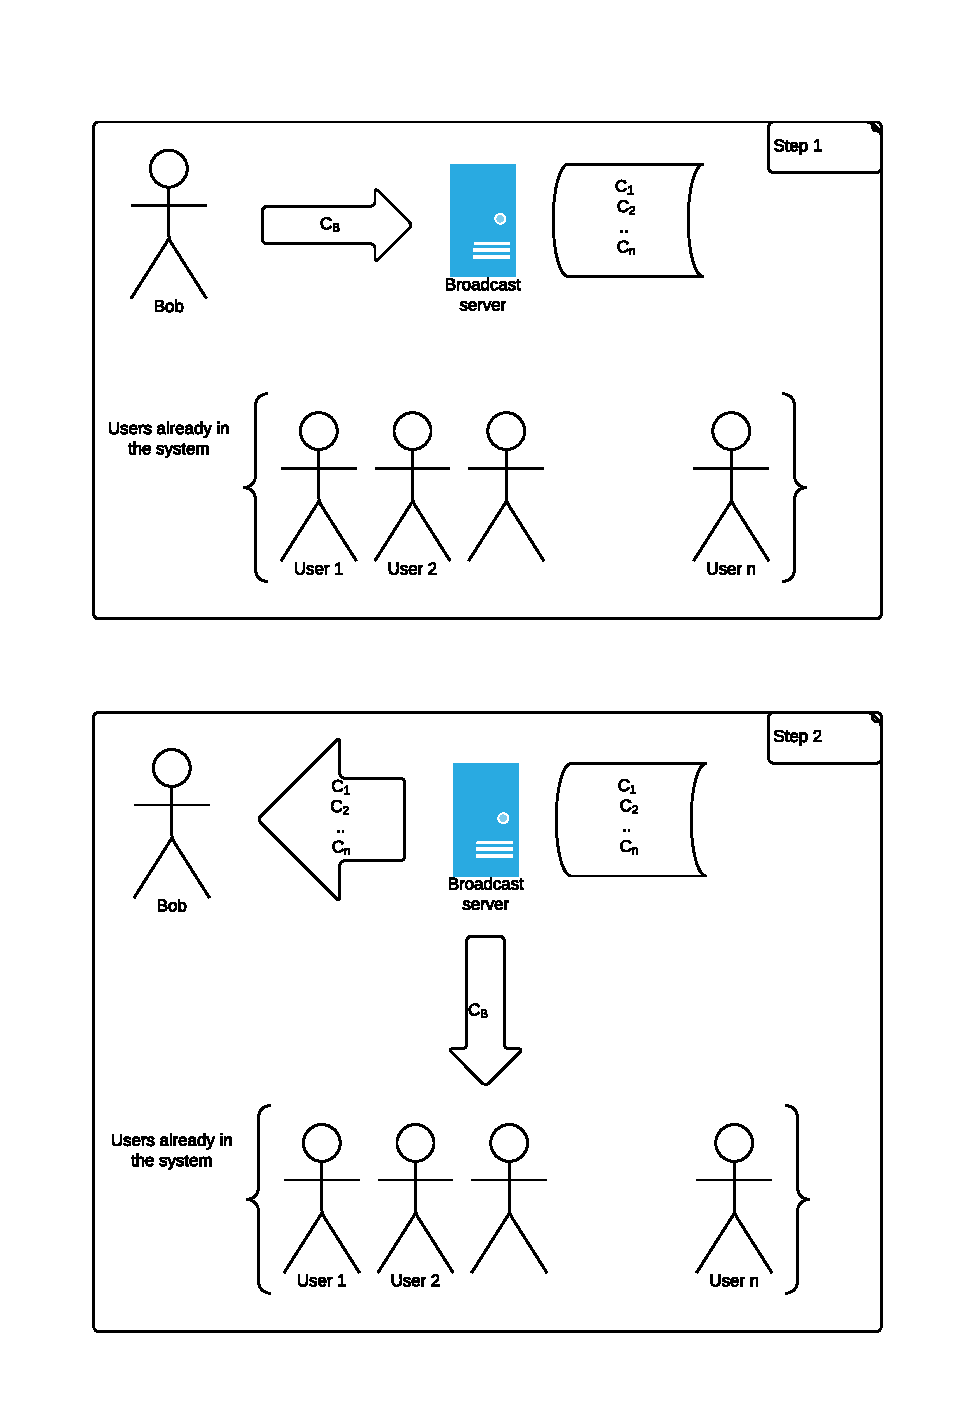
\includegraphics[trim=2cm 1.5cm 2cm 4cm ,scale=1]{chatsystem.pdf}
\caption{Distribution of encapsulations}
\label{fig:encapdistr}
\end{figure}

\begin{figure}
\centering
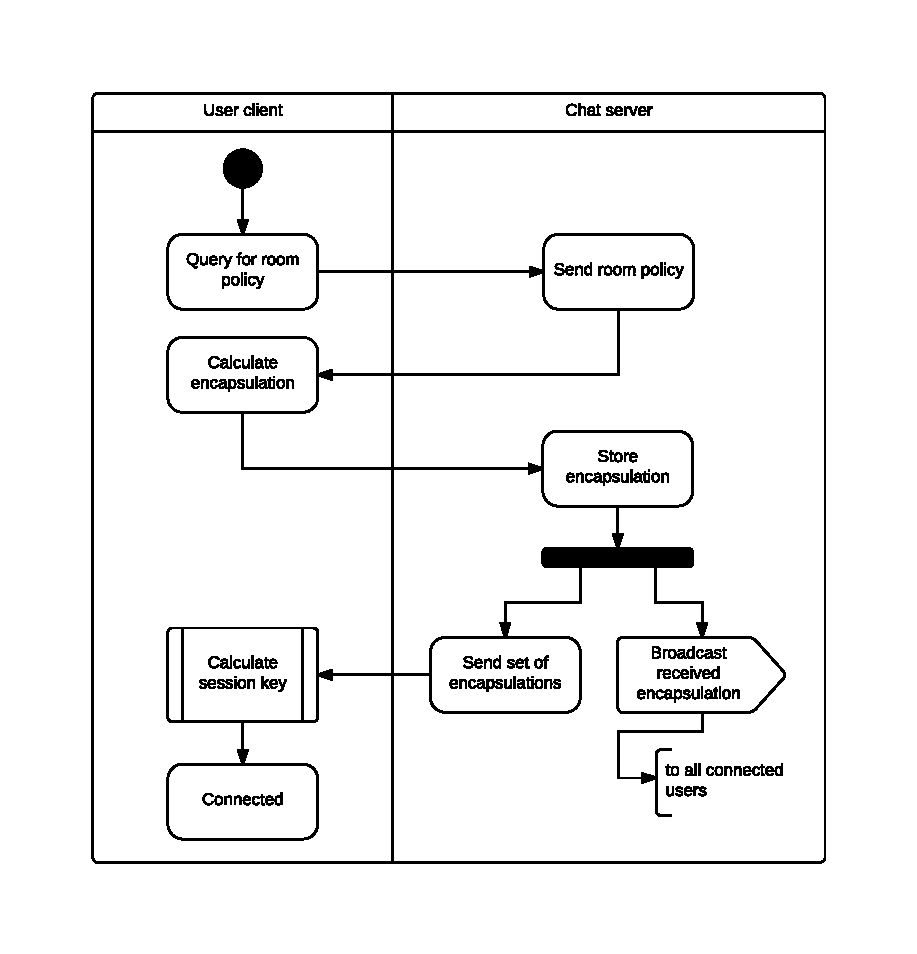
\includegraphics[trim=2cm 2cm 0cm 1cm ,scale=1]{Flow.pdf}
\caption{System flow.}
\label{fig:flow}
\end{figure}
\section{Implementation}
\section{System demonstration}


